\documentclass[12pt,a4paper]{report}
\usepackage{amssymb}
\usepackage{amsthm}
\usepackage{amsmath}
\usepackage{enumitem}
\usepackage{graphicx}
\usepackage{tikz}
\usetikzlibrary{plotmarks}
\usetikzlibrary{patterns,shapes.arrows}
\usepackage{pgfplots}


\DeclareMathOperator{\spn}{span}

\begin{document}
	
\section*{P1: Solve Laplace`s equation on the unit square}

Solve the equation
\begin{align}
\label{equation}
- \Delta u(x, y) = f(x, y),& \quad (x, y) \in \Omega = [0, 1] \times [0, 1] \\
\label{dirch}
u(x, y) = u_\mathcal{D},& \quad (x, y) \in \partial\Omega_{\mathcal{D}} \subset \partial\Omega\\
\label{neum}
\frac{d u(x, y)}{d\mathbf{n}} = g_\mathcal{N},& \quad (x, y) \in \partial\Omega_{\mathcal{N}} = \partial\Omega / \partial \Omega_\mathcal{D}
\end{align}
using a linear approximation finite element approach.

\subsection*{Weak form}
Define a space of test-functions $V$ where $V = \{v | v\in L^2, v(x, y)=0, (x, y) \in \partial \Omega_\mathcal{D}\}$. Multiplying equation \eqref{equation} with $v \in V$ and integrating over the domain yields
\begin{align}
    \int_{\Omega} \Delta u v dx + \int_\Omega f v dx = 0.
\end{align}
Integration by parts and using the fact that $v = 0$ on the Dirichlet boundary gives us
\begin{align}
- \int_{\Omega} \nabla u \cdot \nabla v dx + \int_{\partial\Omega_\mathbf{N}} (\nabla u \cdot n) v ds + \int_\Omega f v dx = 0
\end{align}
where the Neumann boundary condition becomes part of the right-hand-side
\begin{align}
\label{weakform}
\int_{\Omega} \nabla u \cdot \nabla v dx = \int_{\partial\Omega_\mathbf{N}} g_\mathcal{N} v ds + \int_\Omega f v dx.
\end{align}

\subsection*{Grid}

The domain $[0, 1] \times [0, 1]$ is divided into a Cartesian grid with cell width $\Delta x$. Triangle elements are constructed by splitting each cell from the top left to the bottom right corner to make right angled triangles. The reference element is a right triangle with the right corner in $(0, 0)$, the second in $(0, 1)$ and the third in $(1, 0)$. All affine functions over the element can be constructed from linear combinations of the three basis functions
\begin{align}
    \tilde{\phi}_1(x, y) = 1 - x - y \\
    \tilde{\phi}_2(x, y) = x \\
    \tilde{\phi}_3(x, y) = y
\end{align}
where each function is nonzero in only one of the element`s corners (nodes). \\

Using the fact that every element in the grid can be mapped to the reference element by an affine transformation lets the reference element basis functions define functions $\phi_j$ in every element in the grid, creating a basis in the whole domain. Enforcing continuity between elements "fuses" the basis functions that are nonzero in the same node to "hat" functions $\psi_{i}(x, y) = \sum_{n_i} \phi_{n_i}(x, y)$ where $n_i$ runs over the set of $\phi_j$ that are nonzero in the node $i$. These linearly independent functions defines our finite element basis.

\section*{System}

$u,f,g_\mathcal{N}$ in equation \eqref{weakform} are approximated using the finite element basis functions defined above. The approximations are obtained by interpolation. Requiring that the integral equation holds for every $v \in \spn\{\psi_1\ldots\psi_N\}$ transforms the weak form into a linear algebraic equation
\begin{align}
    \label{system}
    \mathbf{A}_0\mathbf{u}_0 = \mathbf{M}_0\mathbf{f}_0 + \mathbf{M}_0^b \mathbf{g}_0
\end{align}
in terms of the approximation coefficients. Where
\begin{align}
    A_{ij} = \int_{\Omega} \nabla \psi_i \cdot \nabla \psi_j dx
\end{align}
defines the stiffness matrix $\mathbf{A}_0$. $\mathbf{M}_0$ and $\mathbf{M}_0^b$ are defined similarly.\\

\subsection*{Dirichlet boundary}
$\mathbf{u}_0$ is not unique without adding a Dirichlet boundary condition. It is enforced by splitting $\mathbf{u}_0= \tilde{\mathbf{u}} + \tilde{\mathbf{u}}_\mathcal{D}$ where $\tilde{\mathbf{u}}_\mathcal{D}$ contains only the coefficients connected to nodes on $\partial\Omega_\mathcal{D}$. The Dirichlet boundary value $u_\mathcal{D}(x, y)$ is then interpolated using the coefficients $\tilde{\mathbf{u}}_\mathcal{D}$. Replacing $\mathbf{u}_0$ in equation \eqref{system} gives us
\begin{align}
\label{system_full}
\mathbf{A}_0 \tilde{\mathbf{u}} = \mathbf{M}_0\mathbf{f}_0 + \mathbf{M}_0^b \mathbf{g}_0 - \mathbf{A}_0 \tilde{\mathbf{u}}_\mathcal{D}.
\end{align}
Reformulating the equation only in terms of the unknowns in $\tilde{\mathbf{u}}$ (ignoring the rows that are 0) lets the equation above be rewritten as 
\begin{align}
\label{system_fin}
\mathbf{A} \mathbf{u} = \mathbf{r}_{f,g,d}.
\end{align}


\subsection*{Convergence test}
To measure convergence rate, the problem is solved for a rhs with known solution, and the $l_2$ error is measured for different $\Delta x$. The error is calculated as 
\begin{equation}
    l_2^{err}(\mathbf{u}) = \sqrt{\sum_i \Delta x^2 (u_i - \bar{u}(x_i, y_i))^2}
\end{equation} where $\mathbf{u}$ is the coefficient vector defined in equation \eqref{system_fin} and $\bar{u}$ is the known solution. $x_i, y_i$ are the coordinates of the node associated with the coefficient $u_i$. The rhs used is
\begin{align}
\bar{f}(x, y) = \sin{\pi y^2}(2\pi \cos{\pi x^2} - 4 \pi x^2 \sin{\pi x^2}) \\
\nonumber
 + \sin{\pi x^2}(2 \pi \cos{\pi y^2} - 4 \pi y^2 \sin{\pi y^2})
\end{align}
with known solution
\begin{align}
\bar{u} = \sin{\pi x^2}\sin{\pi y^2}.
\end{align}


\begin{figure}
	\centering
	% This file was created with tikzplotlib v0.9.15.
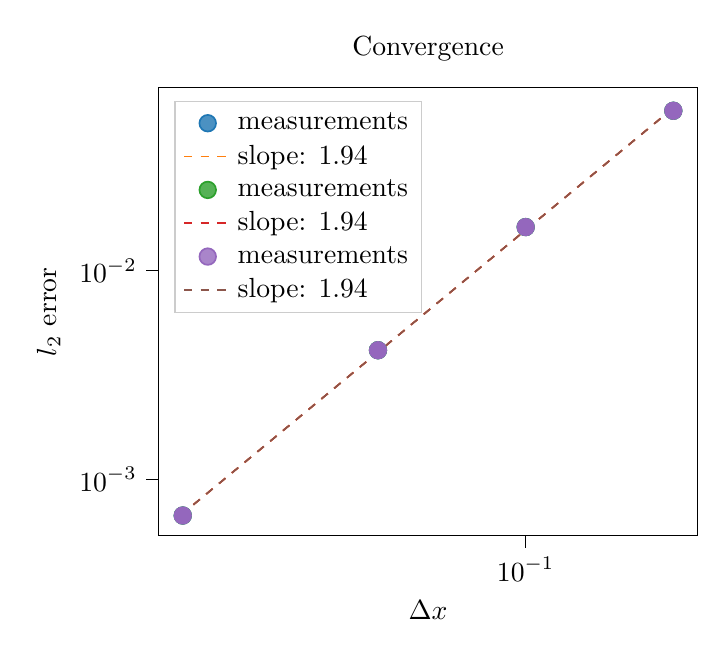
\begin{tikzpicture}

\definecolor{color0}{rgb}{0.12156862745098,0.466666666666667,0.705882352941177}
\definecolor{color1}{rgb}{1,0.498039215686275,0.0549019607843137}
\definecolor{color2}{rgb}{0.172549019607843,0.627450980392157,0.172549019607843}
\definecolor{color3}{rgb}{0.83921568627451,0.152941176470588,0.156862745098039}
\definecolor{color4}{rgb}{0.580392156862745,0.403921568627451,0.741176470588235}
\definecolor{color5}{rgb}{0.549019607843137,0.337254901960784,0.294117647058824}

\begin{axis}[
legend cell align={left},
legend style={
  fill opacity=0.8,
  draw opacity=1,
  text opacity=1,
  at={(0.03,0.97)},
  anchor=north west,
  draw=white!80!black
},
log basis x={10},
log basis y={10},
tick align=outside,
tick pos=left,
title={Convergence},
x grid style={white!69.0196078431373!black},
xlabel={\(\displaystyle \Delta x\)},
xmin=0.0178250187626749, xmax=0.224403690860393,
xmode=log,
xtick style={color=black},
xtick={0.001,0.01,0.1,1,10},
xticklabels={
  \(\displaystyle {10^{-3}}\),
  \(\displaystyle {10^{-2}}\),
  \(\displaystyle {10^{-1}}\),
  \(\displaystyle {10^{0}}\),
  \(\displaystyle {10^{1}}\)
},
y grid style={white!69.0196078431373!black},
ylabel={\(\displaystyle l_2\) error},
ymin=0.000534717996728614, ymax=0.0755424199558287,
ymode=log,
ytick style={color=black},
ytick={1e-05,0.0001,0.001,0.01,0.1,1},
yticklabels={
  \(\displaystyle {10^{-5}}\),
  \(\displaystyle {10^{-4}}\),
  \(\displaystyle {10^{-3}}\),
  \(\displaystyle {10^{-2}}\),
  \(\displaystyle {10^{-1}}\),
  \(\displaystyle {10^{0}}\)
}
]
\addplot [semithick, color0, mark=*, mark size=3, mark options={solid}, only marks]
table {%
0.199999958276749 0.0584786012768745
0.100000001490116 0.0161849036812782
0.0499999932944775 0.00415444374084473
0.0199999958276749 0.000669661036226898
};
\addlegendentry{measurements}
\addplot [semithick, color1, dashed]
table {%
0.199999958276749 0.060319896787405
0.0199999958276749 0.00068475550506264
};
\addlegendentry{slope: 1.94}
\addplot [semithick, color2, mark=*, mark size=3, mark options={solid}, only marks]
table {%
0.199999958276749 0.0584786012768745
0.100000001490116 0.0161849036812782
0.0499999932944775 0.00415444374084473
0.0199999958276749 0.000669661036226898
};
\addlegendentry{measurements}
\addplot [semithick, color3, dashed]
table {%
0.199999958276749 0.060319896787405
0.0199999958276749 0.00068475550506264
};
\addlegendentry{slope: 1.94}
\addplot [semithick, color4, mark=*, mark size=3, mark options={solid}, only marks]
table {%
0.199999958276749 0.0584786012768745
0.100000001490116 0.0161849036812782
0.0499999932944775 0.00415444374084473
0.0199999958276749 0.000669661036226898
};
\addlegendentry{measurements}
\addplot [semithick, color5, dashed]
table {%
0.199999958276749 0.060319896787405
0.0199999958276749 0.00068475550506264
};
\addlegendentry{slope: 1.94}
\end{axis}

\end{tikzpicture}

	\caption{Error decreases approximately $\mathcal{O}(\Delta x^2)$. }
\end{figure}

\subsection*{Solution}
The task was to find the solution for the rhs
\begin{align}
\label{rhs}
f(x, y) = \sin{\pi y^2}(\pi \cos{\pi x^2} - \pi x^2 \sin{\pi x^2}) \\
\nonumber
+ \sin{\pi x^2}(2 \pi \cos{\pi y^2} - 4 \pi y^2 \sin{\pi y^2}).
\end{align}
See figure \ref{solution} for the obtained solution for the above rhs with zero Dirichlet boundary conditions.

\begin{figure}
	\centering
	% This file was created with tikzplotlib v0.9.15.
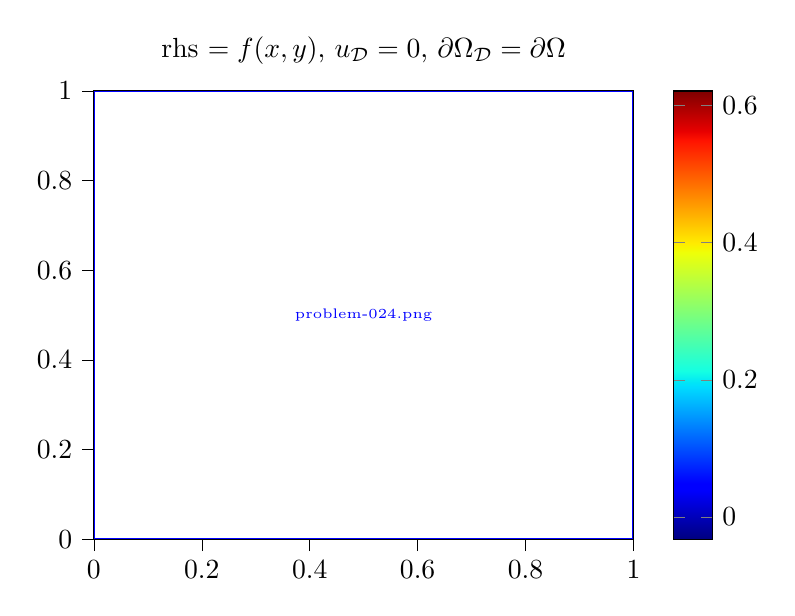
\begin{tikzpicture}

\begin{axis}[
colorbar,
colorbar style={ylabel={}},
colormap={mymap}{[1pt]
  rgb(0pt)=(0,0,0.5);
  rgb(22pt)=(0,0,1);
  rgb(25pt)=(0,0,1);
  rgb(68pt)=(0,0.86,1);
  rgb(70pt)=(0,0.9,0.967741935483871);
  rgb(75pt)=(0.0806451612903226,1,0.887096774193548);
  rgb(128pt)=(0.935483870967742,1,0.0322580645161291);
  rgb(130pt)=(0.967741935483871,0.962962962962963,0);
  rgb(132pt)=(1,0.925925925925926,0);
  rgb(178pt)=(1,0.0740740740740741,0);
  rgb(182pt)=(0.909090909090909,0,0);
  rgb(200pt)=(0.5,0,0)
},
point meta max=0.621352818964573,
point meta min=-0.0323834725094387,
tick align=outside,
tick pos=left,
title={rhs \(\displaystyle =f(x, y)\), \(\displaystyle u_\mathcal{D} = 0\), \(\displaystyle \partial\Omega_\mathcal{D}= \partial \Omega\)},
x grid style={white!69.0196078431373!black},
xmin=0, xmax=1,
xtick style={color=black},
y grid style={white!69.0196078431373!black},
ymin=0, ymax=1,
ytick style={color=black}
]
\addplot graphics [includegraphics cmd=\pgfimage,xmin=0, xmax=1, ymin=0, ymax=1] {problem-024.png};
\end{axis}

\end{tikzpicture}

	\caption{\label{solution}Solution to the PDE with rhs from equation \eqref{rhs}.}
\end{figure}

\begin{figure}
	\centering
	% This file was created with tikzplotlib v0.9.15.
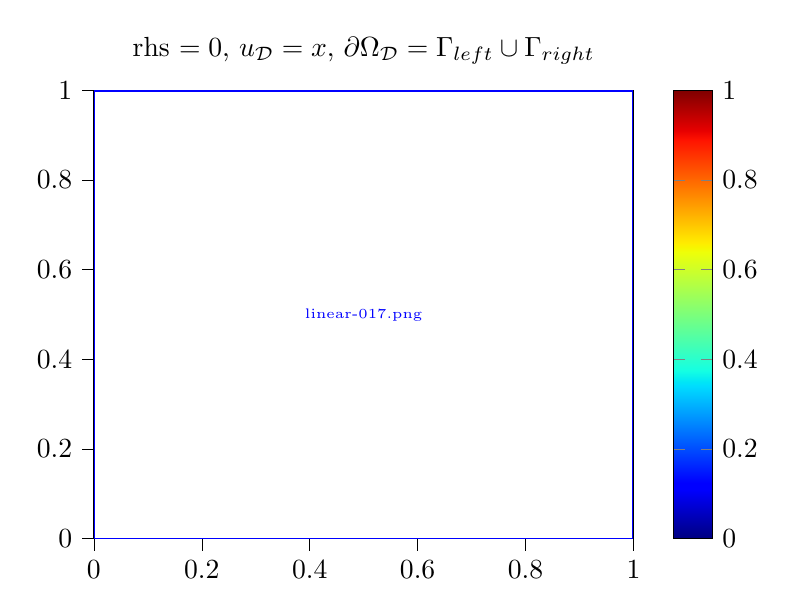
\begin{tikzpicture}

\begin{axis}[
colorbar,
colorbar style={ylabel={}},
colormap={mymap}{[1pt]
  rgb(0pt)=(0,0,0.5);
  rgb(22pt)=(0,0,1);
  rgb(25pt)=(0,0,1);
  rgb(68pt)=(0,0.86,1);
  rgb(70pt)=(0,0.9,0.967741935483871);
  rgb(75pt)=(0.0806451612903226,1,0.887096774193548);
  rgb(128pt)=(0.935483870967742,1,0.0322580645161291);
  rgb(130pt)=(0.967741935483871,0.962962962962963,0);
  rgb(132pt)=(1,0.925925925925926,0);
  rgb(178pt)=(1,0.0740740740740741,0);
  rgb(182pt)=(0.909090909090909,0,0);
  rgb(200pt)=(0.5,0,0)
},
point meta max=1,
point meta min=0,
tick align=outside,
tick pos=left,
title={rhs \(\displaystyle =0\), \(\displaystyle u_\mathcal{D} = x\), \(\displaystyle \partial\Omega_\mathcal{D}= \Gamma_{left} \cup \Gamma_{right} \)},
x grid style={white!69.0196078431373!black},
xmin=0, xmax=1,
xtick style={color=black},
y grid style={white!69.0196078431373!black},
ymin=0, ymax=1,
ytick style={color=black}
]
\addplot graphics [includegraphics cmd=\pgfimage,xmin=0, xmax=1, ymin=0, ymax=1] {linear-017.png};
\end{axis}

\end{tikzpicture}

	\caption{Experiment with nonzero Dirichlet boundary.}
\end{figure}

\begin{figure}
	\centering
	% This file was created with tikzplotlib v0.9.15.
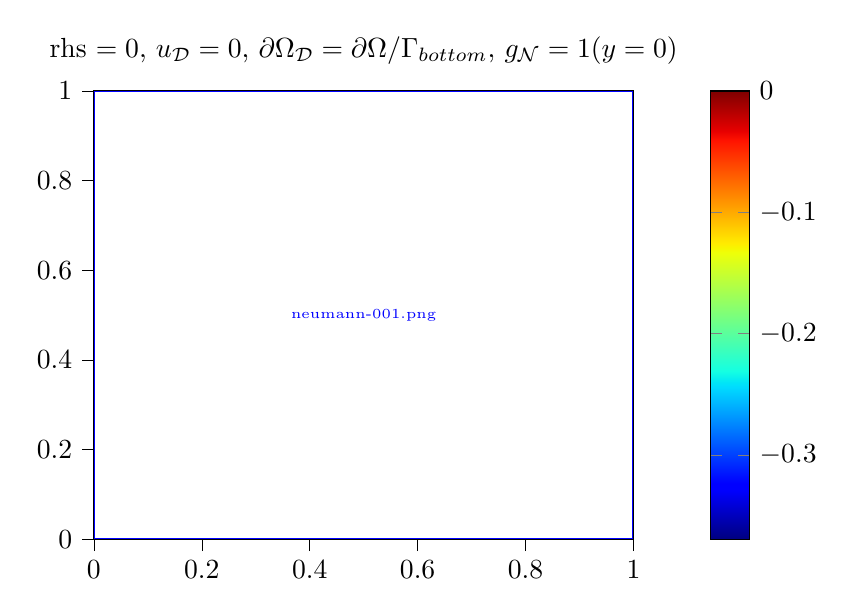
\begin{tikzpicture}

\begin{axis}[
colorbar,
colorbar style={ylabel={}},
colormap={mymap}{[1pt]
  rgb(0pt)=(0,0,0.5);
  rgb(22pt)=(0,0,1);
  rgb(25pt)=(0,0,1);
  rgb(68pt)=(0,0.86,1);
  rgb(70pt)=(0,0.9,0.967741935483871);
  rgb(75pt)=(0.0806451612903226,1,0.887096774193548);
  rgb(128pt)=(0.935483870967742,1,0.0322580645161291);
  rgb(130pt)=(0.967741935483871,0.962962962962963,0);
  rgb(132pt)=(1,0.925925925925926,0);
  rgb(178pt)=(1,0.0740740740740741,0);
  rgb(182pt)=(0.909090909090909,0,0);
  rgb(200pt)=(0.5,0,0)
},
point meta max=0,
point meta min=-0.369414712324147,
tick align=outside,
tick pos=left,
title={rhs \(\displaystyle =0\), \(\displaystyle u_\mathcal{D} = 0\), \(\displaystyle \partial\Omega_\mathcal{D}= \partial \Omega / \Gamma_{bottom} \), \(\displaystyle g_\mathcal{N} = 1(y=0)\)},
x grid style={white!69.0196078431373!black},
xmin=0, xmax=1,
xtick style={color=black},
y grid style={white!69.0196078431373!black},
ymin=0, ymax=1,
ytick style={color=black}
]
\addplot graphics [includegraphics cmd=\pgfimage,xmin=0, xmax=1, ymin=0, ymax=1] {neumann-001.png};
\end{axis}

\end{tikzpicture}

	\caption{Experiment with Neumann boundary.}
\end{figure}

\section*{P2: Classify the equations}
\begin{enumerate}[label=\alph*]
	\item Scalar nonlinear time dependent PDE.
	\item Scalar second order ODE.
	\begin{itemize}
		\item Example initial value: $u(0) = 0$.
	\end{itemize}
	\item Vector valued linear ODE.
	\begin{itemize}
	    \item Example initial value: $\mathbf{u}(-1) = \mathbf{0}$.
    \end{itemize}
	\item Linear algebraic equation system.
	\item A system of time dependent PDE:s describing a local conservation law in a one dimensional domain.
	\begin{itemize}
		\item Example equation: 1D Euler equations.
		\item Example initial value: $\mathbf{u}(x, 0) = \mathbf{c}(x), \quad x\in [0, 1]$.
		\item Example Dirichlet boundary condition: $\mathbf{u}(0, t) = \mathbf{c}(t), \quad t\in[0, 1]$.
		\item Example in-flow boundary condition: $\mathbf{f}(\mathbf{u})(0, t) = \mathbf{c}(t), \quad t\in[0, 1]$.
	\end{itemize}
		\item A system of time dependent PDE:s describing a local conservation law. Coupled with a scalar ODE defining a time dependent Dirichlet type boundary condition(?) on the intersection of the non-overlapping regions $\Omega_1$ and $\Omega_2$.
	\begin{itemize}
		\item Example initial value: $\mathbf{u}(\mathbf{x}, 0) = \mathbf{c}(\mathbf{x}), \quad \mathbf{x}\in \Omega_1, \quad y(\mathbf{z}, 0) = h(\mathbf{z}), \quad \mathbf{z} \in \Omega_2$.
		\item Example Dirichlet boundary condition: (together with the condition in the task) $\mathbf{u}(\mathbf{x}, t) \perp \mathbf{n} = \mathbf{0}, \quad \mathbf{x}\in\Omega_1 \cap \Omega_2, \quad t\in[0, 1]$ and $\mathbf{u}(\mathbf{x}, t) = \mathbf{c}(t), \quad \mathbf{x} \in \partial \Omega_1 / \Omega_2, \quad t\in[0, 1]$.
	\end{itemize}
\end{enumerate}


	
\end{document}